i\documentclass[a4paper,12pt]{article}
\addtolength{\oddsidemargin}{-1.cm}
\addtolength{\textwidth}{2cm}
\addtolength{\topmargin}{-3cm}
\addtolength{\textheight}{3.5cm}
\makeindex


\usepackage[pdftex]{graphicx}
\usepackage{makeidx}
\usepackage{float}
\usepackage{hyperref}
\hypersetup{
	colorlinks=true,
	linkcolor=blue,
	filecolor=magenta,      
	urlcolor=cyan,
}



% define the title
\author{CodeBlox}
\title{Tender}
\begin{document}
	\setlength{\parskip}{6pt}
	
	% generates the title
	\begin{titlepage}
		\begin{center}
			
\includegraphics[width=1\textwidth]{./Pictures/up_logo.png}\\[1.5cm] 
			\textsc{\LARGE Department of Computer Science} \\ [.5cm]
			\textsc{\Large Functional and Architectural Requirements} \\ [.5cm]
			\line(1,0){450}\\[.5cm]
			\huge{\bfseries Client: Gavin Potgieter}\\
			\line(1,0){450}\\[.5cm]
			\textsc{\LARGE Team: CodeBlox}\\ [0.5cm]
			
			
			\textsc{\large Tshepo Malesela (Bsc: Computer Science)}\\
			\textsc{\large Lorenzo Spazzoli (Bsc: Computer Science)}\\
			\textsc{\large Bilal Muhammad (BIS: Multimedia)}\\
			\textsc{\large Dirk de Klerk (BIS: Multimedia)}\\ [3.9cm]
			
			\large\today
		\end{center}
	\end{titlepage}
	
	\tableofcontents
	\thispagestyle{empty}
	\footnotesize
	\normalsize
	
	\newpage
	\section{Architectural Requirements/Design Specification}
	
	\subsection{Software architecture overview}
	
	The diagram below provides a high-level overview of the software architecture as a whole. For this particular project we are making use of a Micro Services Architecture, therefore the diagram shows how the respective components of the system will be integrated.\\
	
	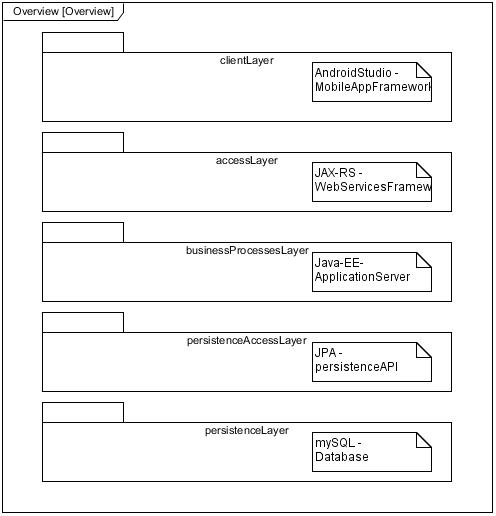
\includegraphics[width=1\textwidth]{./Pictures/UML/architectureOverview.jpg}\\[1.5cm]
	
	
	\subsubsection{The Clients}
	The component with which the client will be interacting. This will represent the interface with which the client will be interacting, be it an android or web interface.
	\subsubsection{API Gateway}
	This component will serve as a single entry point to all the micro services provided by the architecture. The API gateway will be responsible to expose a different API for each of the respective clients. 
	\subsubsection{RESTful layer}
	Each of the respective microservices will be wrapped in a restful layer, which is then accessed and controlled by the API Gateway. 
	\subsubsection{Micro Services}
	The micro services are all of the independent functional components that make up the application as a whole. Each of these services aim to complete/address a single task. i.e. each of the microservices will only have a single responsibility. 
	\subsubsection{Persistence}
	This component is where the microservices will end up storing its information. This particular architecture will make use of a NoSQL database. Each of the microservices will be responsible for maintaining its own persistence as to keep the services decoupled from each other as much as possible.
	
	\subsection{Access Channel Requirements}
	\begin{itemize}
		\item An android application that allows the owner of the property to be notified when someone is outside the premises and to have a full video stream while the person is on the residence.
		
		\item The android application should also allow the owner to remotely provide or refuse access to the premises or dropOff device.
		
		\item The application should also allow the owner to generate/provide the person with an access pin, should the camera feed and remote access system not be available at the time.  
		
		\item Ideally the owner should be able to communicate with the individual/delivery person via voice communication in unison with the camera feed. 
	\end{itemize}
	
	\newpage
	\subsection{Architectural Scope}
	\begin{itemize}
		\item Video stream access of the premises from anywhere at any time i.e. constant camera footage of the premises. This will be done using SIP (Session Initiation Protocol).
		
		\item Voice will also be transmitted using SIP, when the delivery person interacts with the intercom system.
		
		\item An internal server that will host all of the devices within the household, and that will allow additional devices to be appended as needed in the future.
		
		\item An external server that is responsible for establishing communications with the internal server and user application. As well as the responsibility of authenticating and authorizing users. 
	\end{itemize}
	
	\subsection{Quality Requirements}
	
	\subsubsection{Performance}
	\begin{itemize}
		\item The system should respond to user requests within a reasonable amount of time.
		\item The live stream delay from the camera should be kept to minimum (ideally no more than a 1 second delay). 
		\item The same delay times should apply for voice streaming should a intercom system be employed.
	\end{itemize}
	
	\subsubsection{Scalability}
	The systems ability to adapt to change in the number of users and should allow:
	\begin{itemize}
		\item the system to handle an increased amount of traffic.
		\item the amount of resources should be able to be easily increased. 
	\end{itemize}
	
	\subsubsection{Security}
	\begin{itemize}
		\item First and foremost, the system needs to be able to authenticate a user, so that only he/she may access the various services provided.
		\item Secondly the system needs to be able to authorize the user so that he/she may only use the services for which they are registered.
	\end{itemize}
	
	\subsubsection{Privacy}
	Relates to sensitive user information that they would not like exposed and should not:
	\begin{itemize}
		\item reveal any information about a user that is considered sensitive to any improper parties.
	\end{itemize}
	
	\subsubsection{Reliability}
	The system should provide a reasonable level of availability and reliability.
	\begin{itemize}
		\item The system should provide the user with a fail-safe mechanism to still have access to the basic functionality of the system.
		\item Allow deployment of services without affecting the neighboring services. 
	\end{itemize}
	
	\subsubsection{Flexibility}
	\begin{itemize}
		\item One should be able to add additional access channels and devices to the system, which is especially relevant to this particular project.
		\item Add additional functionality to the system with ease.
	\end{itemize}
	
	\subsubsection{Maintainability}
	The system should in future, support maintainability. This will include:
	\begin{itemize}
		\item a system that is easily understood by future developers.
		\item technologies used within the system should have a reasonable lifetime, as to not force a migration to new technologies in future.
		\item adding upgrades to the system with ease and minimum downtime.
	\end{itemize}
	
	\subsubsection{Monitorability}
	Relates to how the system is functioning and should allow:
	\begin{itemize}
		\item operators of the system to monitor its operation from a remote location.  
	\end{itemize}
	
	\subsubsection{Usability}
	Relates to how users will be interacting with the system and should allow:
	\begin{itemize}
		\item the system to be intuitive and efficient to use with the need to provide additional training.
		\item the average android or web user should find the system easy to use.
	\end{itemize}
	
	\subsubsection{Cost}
	\begin{itemize}
		\item The cost of the system should be kept to a minimum and made as affordable as possible.  
	\end{itemize}
	
	\subsubsection{Testability}
	\begin{itemize}
		\item The individual components of the system needs to be testable through the use of mock objects and automated unit tests.
		\item Automated integration tests should be used to test the system as a whole.
		\item In particular the tests need to verify that the preconditions are met, and that post conditions hold true once a service has been provided.
	\end{itemize}
	
	\newpage
	\subsection{Architectural Constraints}
	The client has some architectural specifications in place that will need to be adhered to in order to successfully complete this project.
	
	\subsubsection{Use of Inexpensive Devices}
	The devices used to construct the physical system needs to be as inexpensive as possible, thus providing a larger audience with access to it. Devices such as the following will be included:
	\begin{itemize}
		\item Raspberry Pi 3
		\item IP Camera/Pi Camera
		\item Internet Enabled Switches
		\item WiFi Routers
		\item Android Smartphone (Users are assumed to posses one already).
	\end{itemize}
	
	\subsubsection{Technology Stack}
	For monetary reasons, the client has requested that the entire system be developed using open source technologies. CodeBlox has therefore decided to settle on a JavaScript Ecosystem, since it addresses performance and scalability requirements intrinsically through the use of the MEAN stack. The MEAN stack refers to MongoDB, Expressjs, Angularjs, Nodejs. A Preliminary stack will include the following technologies:
	
	\begin{itemize}
		\item \textbf{JavaScript} The primary language to be used throughout the development of the system.
		\item \textbf{Nodejs and Express.js} as the cross-platform runtime environment that supports the creation of new modules using JavaScript. Express will also have the responsibility of making the services RESTful. 
		\item \textbf{Android Studio} to the build the mobile application that will be used.
		\item \textbf{npm Scripts} will be used as the primary build tool and will be in charge of keeping track of the life cycle.
		\item \textbf{Mocha and Chai} will be used for unit testing and assertion
		\item \textbf{JAX-RS} for implementing RESTful webservices.
		\item \textbf{Linux} as the operating system
		\item \textbf{MongoDB} as the primary persistence technology.
		\item \textbf{Mongoose} as an ODM to provide additional functionality when working with MongoDB.
		\item \textbf{AngularJS} as the primary framework for developing a web application.
		\item \textbf{Heroku} will be used to host the application online.
	\end{itemize}
	
	\newpage
	\subsection{Architectural Design}
	This section specifies the architectural responsibilities of various architectural components.
	\subsubsection{Architectural Responsibilities}
	\begin{itemize}
		\item The responsibility of providing an execution environment for business processes is assigned to an application server. i.e. \textbf{Nodejs/Express} itself.
		\item The responsibility of persisting domain objects is assigned to the the database i.e. \textbf{MongoDB}
		\item The responsibility of providing access to the database and converting between POJO's and JSON is left to the ODM i.e. \textbf{Mongoose}
		\item The responsibility of providing access channels to users is assigned to the web services framework i.e. \textbf{Express.js}
		\item The responsibility of providing users access via mobile devices is assigned to the mobile application framework i.e. \textbf{Android Studio}
	\end{itemize}
	
	\subsubsection{Infrastructure}
	For this particular project, the \textbf{Microservices architectural pattern} will be used as an infrastructure. Although no clear definition exists for the pattern it can be described in terms of it attributes:
	\begin{itemize}
		\item \textbf{Software can be broken down into multiple component services.} Thus each service can be deployed, tweaked, and redeployed independently.
		\item \textbf{Services are organised around business capabilities and priorities.} Thus each team/member can develop and maintain services independently.
		\item \textbf{Functions like a classical UNIX system.} Thus it receives requests, processes them and responds to them accordingly.
		\item \textbf{Favours decentralised governance over centralised governance.} Allows developers to produce useful tools that can be used by others to solve the same problem; use existing tools to solve own problems; Each service manages its own unique database.
		\item \textbf{Designed to cope with failure.} Neighbouring services should continue to function independently of the failed service.
		\item \textbf{Focusses on evolutionary design.} This is extremely useful when you can't anticipate the types of devices that may need to access your application in future.
	\end{itemize}
	
	\newpage
	\subsection{Application Server/Micro Services}
	The Micro Services component of the architecture is where all the business logic of the system will hosted. Each of the services within the system will address as specialised need/function. The Micro Services themselves will be implemented via Nodejs/Expressjs.
	
	\subsubsection{Quality Requirements}
	\begin{itemize}
		\item\textbf{Performance}
		\begin{itemize}
			\item The system should respond to user requests within a reasonable amount of time.
		\end{itemize}
		
		\item\textbf{Scalability}
		\begin{itemize}
			\item The server should be able to cope with a reasonable increase in the amount of users using the system for the amount of resources available. 
		\end{itemize}
		
		\item\textbf{Maintainability}
		\begin{itemize}
			\item The system should be easily maintainable by future developers with as little downtime as possible. 
		\end{itemize}
		
		\item\textbf{Flexibility}
		\begin{itemize}
			\item New functionality/services should be able to be deployed independently of other existing services.
		\end{itemize}
		
		\item\textbf{Reliability}
		\begin{itemize}
			\item Requires that service requests are not partially executed. Thus the requested service will only be executed once postconditions are fulfilled. If a service could not be provided, a reason must be given.
		\end{itemize}
		
		\item\textbf{Security}
		\begin{itemize}
			\item The application server must support role-based authorisation. Thus only a user with a certain level of authorisation may execute certain processes. No direct access should be provided to the database. 
		\end{itemize}
		
		\item\textbf{Testability}
		\begin{itemize}
			\item The application server should support out-of-container testing as well as unit testing.
		\end{itemize}
		
	\end{itemize}
	
	\newpage
	\subsubsection{Tactics as provided by Nodejs and Micro Services Architecture}
	Node.js/Expressjs and the Micro Services Architecture itself, address the quality requirements mentioned above intrinsically.
	
	\begin{itemize}
		\item\textbf{Performance Tactics}
		\begin{itemize}
			\item The Node.js Runtime Environment interprets JavaScript using Google’s V8 JavaScript Engine. The engine compiles JavaScript to native machine code before executing it, instead of using more traditional means such as interpreting the code to provide increased performance.
		\end{itemize}
		
		\item\textbf{Scalability Tactics}
		\begin{itemize}
			\item Node.js has an event-driven architecture capable of asynchronous I/O. This allows the creation of highly scalable servers without using threading, by using events-driven programming that uses callbacks to signal the completion of a task. This architecture aims to optimize scalability in web applications containing many I/O operations, as well as real-time Web applications. 
		\end{itemize}
		
		\item\textbf{Maintainability Tactics}
		\begin{itemize}
			\item Since the Micro Services Architecture focusses on dividing the application into functional services, it inherently improves maintainability by allowing modules to be modifies and redeployed independently.
			\item Nodejs uses a modular approach to programming that supports this architectural pattern. 
		\end{itemize}
		
		\item\textbf{Flexibility Tactics}
		\begin{itemize}
			\item The independence of each service as well as micro services' tendency to favour decentralised governance, mean that new functionality can be added without affecting the existing services.
			\item The notion of evolutionary design is another factor that improves the systems ability to be flexible.
		\end{itemize}
		
		\item\textbf{Reliability Tactics}
		\begin{itemize}
			\item Each service of the system should be executed in full once each of the preconditions have been met. If such a service can not be provide, a suitable reason must be given/exception thrown.
		\end{itemize}
		
		\item\textbf{Security Tactics}
		\begin{itemize}
			\item The provide the system with sufficient security. His/Her user credential will be exchanged for that of a JSON Web Token (JWT), which will then be saved locally. This token is then used for all future transactions and will be sent with every request.
		\end{itemize}
		
		\newpage
		\item\textbf{Testability Tactics}
		\begin{itemize}
			\item The Mocha and Chai npm modules provide a comprehensive testing framework and assertion library. Used with npm Scripts, a fully automated unit and integration test suite can be developed that can be executed as part of the build life cycle of the system. 
		\end{itemize}
		
	\end{itemize}
	
	\newpage
	\subsection{Persistence}
	For this particular project we will be utilising a non-relational database, namely \textbf{MongoDB}. MongoDB is a free and open-source cross-platform, document-oriented database. Classified as a NoSQL database, MongoDB avoids the traditional table-based relational database structure in favour of JSON-like documents with dynamic schemas. 
	
	\subsubsection{Quality Requirements}
	\begin{itemize}
		\item\textbf{Performance}
		\begin{itemize}
			\item The database should return the necessary information/JSON objects within a reasonable amount of time.
		\end{itemize}
		
		\item\textbf{Scalability}
		\begin{itemize}
			\item The database should support horizontal scaling across an array of hardware to cope with an increased number of users. 
		\end{itemize}
		
		\item\textbf{Security and Privacy}
		\begin{itemize}
			\item The information stored within the database should be secure at all times.
			\item Sensitive user information should be kept private from unauthorised parties.
		\end{itemize}
		
		\item\textbf{Accessibility}
		\begin{itemize}
			\item The required information should be easily accessible from the database.
		\end{itemize}
		
		\item\textbf{Availability}
		\begin{itemize}
			\item The data should always be available for retrieval and use.
		\end{itemize}
	\end{itemize}
	
	\subsubsection{Tactics as provided by MongoDB}
	MongoDB addresses many of the quality requirements intrinsically through the way it has been designed and implemented.
	
	\begin{itemize}
		\item\textbf{Performance and Scalability Tactics}
		\begin{itemize}
			\item MongoDB is a NoSQL database, particularly a document-oriented database. These databases assume that documents encapsulate and encode data in some standard format, in this case binary forms of JSON. NoSQL databases include some forms of sharding/partitioning which enables them to be scaled out on hardware (servers) or the cloud. This provides them with massive scalability potential, as well as higher throughput and lower latency, hence improved performance. 
		\end{itemize}
		
		\item\textbf{Security and Privacy Tactics}
		\begin{itemize}
			\item To be a completed.
		\end{itemize}
		
		\item\textbf{Accessibility Tactics}
		\begin{itemize}
			\item MongoDB avoids the traditional table-based relational database structure and uses JSON-like documents with dynamic schemas instead. This makes the integration of data in certain applications easier and faster. Thus it provides developers with an easier way of storing and accessing data since “fields” can vary dynamically. Mongoose ODM is used to store objects within the MongoDB database. 
		\end{itemize}
		
		\item\textbf{Availability Tactics}
		\begin{itemize}
			\item MongoDB provides a user with Automatic Failover. This is the process of switching operations to a redundant or standby server or hardware component, if the primary server or component failed for some reason. This will ensure that the data required by the system will always be available.
		\end{itemize}
	\end{itemize}
	
	\newpage
	\subsection{Mongoose}
	Mongoose is a Node.js library that provides MongoDB with Object Document Mapping, which is the ORM version of non-relational document-oriented databases. Mongoose translates data in the database to JavaScript objects for use in the application and vice versa.
	
	{\noindent}Additional Quality requirements addressed by Mongoose:
	\begin{itemize}
		\item \textbf{Reduction in code bulk:} ODM provides numerous services thereby allowing the developer to focus on the creation of business logic as opposed to writing repetitive database queries. 
		\item \textbf{Changes to object model are made in one place.} Once an update has been made to object definitions, the ODM will automatically use the updated model for future queries. 
		\item \textbf{Caching.} Entities are cached in memory thereby reducing the load on the database. 
	\end{itemize}
	
	\newpage
	\subsection{RESTful Webservices}
	REST is an architectural style for networked hypermedia applications, it is primarily used to build Web services that are lightweight, maintainable, and scalable. A service based on REST is called a RESTful service. REST is not dependent on any protocol, but almost every RESTful service used HTTP as its underlying protocol.
	
	\noindent Every system uses resources and these resources can take the form of any media. The purpose of a service is to provide a window to its clients so that they can access these resources i.e. expose these resources.
	
	\noindent RESTful sevices should have the following properties:
	
	\begin{itemize}
		\item Representations
		\item Messages
		\item URI's
		\item Uniform interface
		\item Stateless
		\item Links between resources
		\item Caching
	\end{itemize}
	
	\noindent RESTful sevices will be implemented via the Node Express.js library.
	
	\subsubsection{API Gateway}
	The API Gateway enables the system to expose a different API for each client. This will enable control over which services are available to which user in the context of which services have been paid for. The API Gateway can also be used to implement security in terms of verifying that a client is authorized to perform the request.
	
	\subsubsection{Client - Web}
	Still under revision - To be implemented using AngularJS.
	\subsubsection{{Client - Android App}}
	Still under revision - To be implemented using Android Studio.
\end{document}
